\subsection{Wechselstrom-Schalter/Steller}
\subsubsection{Wechselstrom-Schalter}
\begin{minipage}{0.6\linewidth}
    Wegen dem Polaritätswechel besteh der Wechselstromschalter aus zwei antiparallelen Thyristoren, welche die Stromhalbschwingung abwechselnd ausführen.
\end{minipage}

\begin{minipage}{0.3\linewidth}
    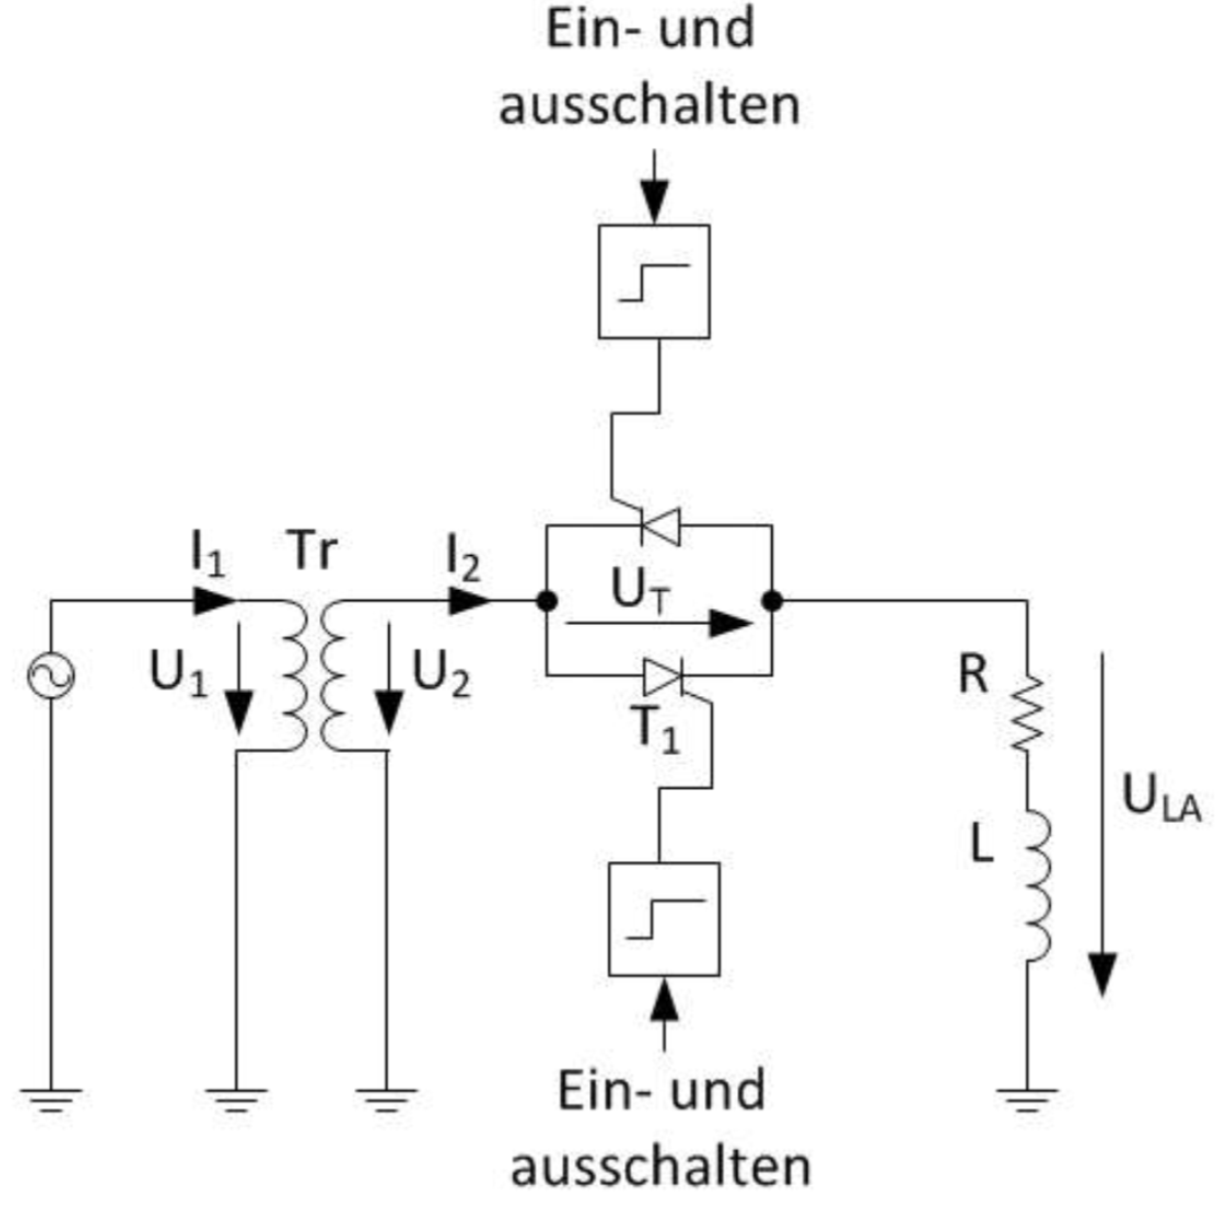
\includegraphics[width=\linewidth]{images/SchemaWSSchalter}
\end{minipage}
\begin{minipage}{0.3\linewidth}
    \textbf{Lasttyp: R}\newline
    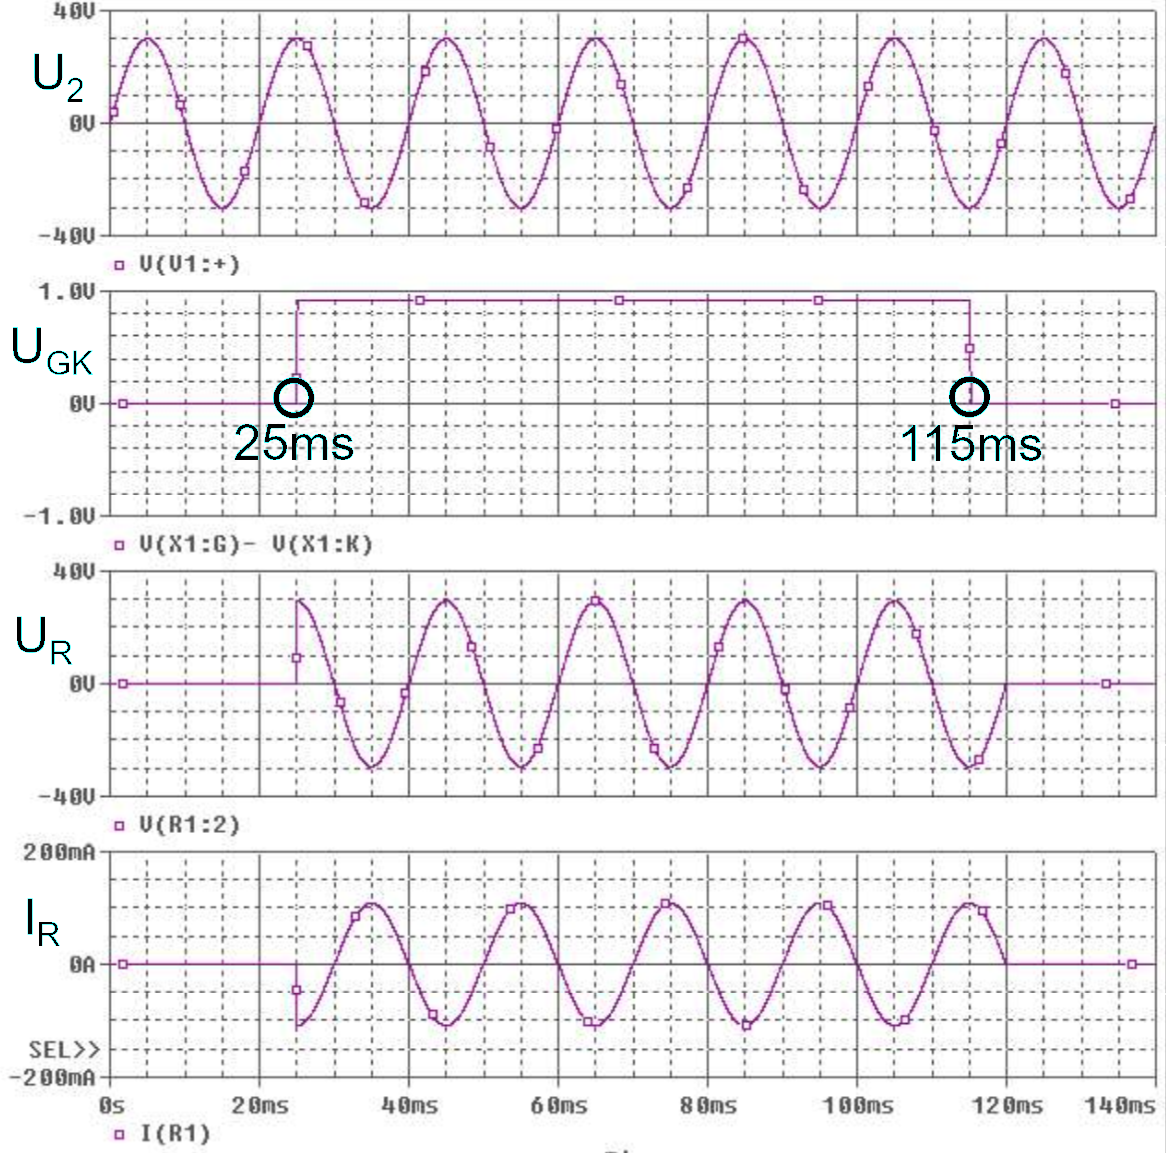
\includegraphics[width=\linewidth]{images/KLWSSchalter}
\end{minipage}
\begin{minipage}{0.3\linewidth}
    \textbf{Lasttyp: R + L}\newline
    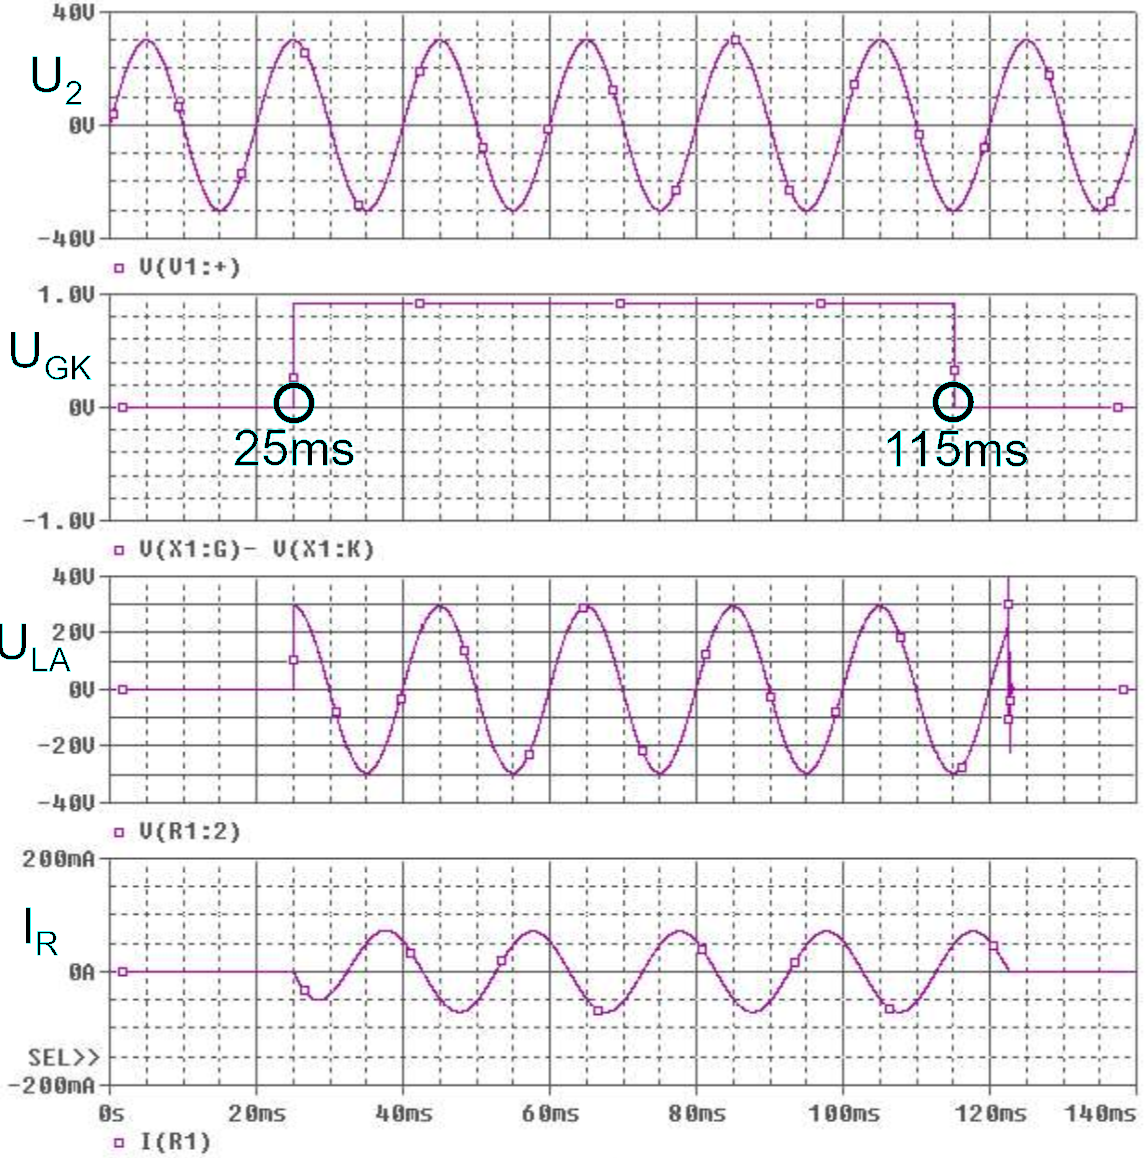
\includegraphics[width=\linewidth]{images/KLWSSchalter2}
\end{minipage}






\subsubsection{Wechselstrom-Steller}


\clearpage